\section{Extended Kalman Filter}
\label{extended_kalman_filter}

All of  our discussion to this point has considered linear filters for linear systems.
Unfortunately, linear systems do not  exist.  All systems are ultimately nonlinear.

However, many systems are  close enough to linear that linear estimation approaches give satisfactory results. 
But  close enough can only be carried so far.  Eventually, we run across a system 
that does not behave linearly even over a small range of  operation, and our linear 
approaches for  estimation  no longer give good results.  In this case, we  need  to  explore nonlinear estimators. 

In this section, we will discuss some nonlinear extensions of  the Kalman filter. 
The Kalman filter  that we  discussed earlier, applies only to 
linear  systems.  However,  a  nonlinear  system  can  be  linearized, and then  linear  estimation  techniques  (such  as the  Kalman  or  $H_{\infty}$, 
filter) can be applied.  



%\subsection{The Linearized Kalaman Filter }
%\label{linearized_kalman_filter}
%In  this section, we  will show how  to linearize a nonlinear system, and  then  use 
%Kalman  filtering theory to estimate the  deviations  of  the state  from a  nominal 
%state value. This will then give us an estimate of the state of the nonlinear system.

%We will derive the linearized Kalman filter from the continuowtime viewpoint, but 
%the analogous derivation for discretetime or hybrid systems are straightforward.

\subsection{The Extended Kalman Filter }
\label{extended_kalman_filter}

%The previous section obtained a linearized Kalman filter for estimating the states of 
%a nonlinear system.  The derivation was based on linearizing the nonlinear system 
%around a nominal state trajectory.  The question that arises is, How do we know 
%the nominal state trajectory? 

In some cases it may not be straightforward to find 
the nominal trajectory.  However, since the Kalman  filter estimates the state of 
the system, we can use the Kalman filter estimate as the nominal state trajectory.

This is sort of a bootstrap method.  We linearize the nonlinear system around the 
Kalman filter estimate, and the Kalman filter estimate is based on the linearized 
system. This is the idea of the extended Kalman filter (EKF), which was originally 
proposed by Stanley Schmidt so that the Kalman filter could be applied to nonlinear 
spacecraft navigation problems.

\begin{framed}
\theoremstyle{remark}
\begin{remark}{\textbf{EKF and IEKF}}

Now this filter comes in two versions, you might say,
the normal one and then as an iterative solution
similar to what we do when we solve an optimization problem using a Gauss Newton search.
The basic idea is simple and natural. if we have nonlinear models $\mathbf{f}_{k-1}$ and $\mathbf{h}_k$,
why don't we simply linearize these? This will lead us to linear models and we know how to handle these.
\end{remark}
\end{framed}

So in the prediction step we linearize our nonlinear motion
model around our posterior estimate
from the previous time instance and use a normal Kalman filter prediction.

Now why do we use the posterior mean
from the previous time instance as our linearaziation point?
Well, our motion model $\mathbf{f}$ is a function of $\mathbf{x}_{k-1}$. Our best guess of what $\mathbf{x}_{k-1}$
is when we do the prediction is our posterior mean.
So naturally, we want our linearization to be as accurate as possible, at or near where we
think $\mathbf{x}_{k-1}$ actually is.

Now for the update step, we basically do the same thing.
When we linearize $\mathbf{h}_{k}(\mathbf{x}_k$, but as the measurement model
is a function of $\mathbf{x}_k$, we use our predicted estimate, $\hat{\mathbf{x}}_{k|k-1}$ as our linearization point,
and then use the Kalman filter update with this linearized model.

However, the linear Kalman filter cannot be used directly
to estimate states that are nonlinear functions of either
the measurements or the control inputs. For example, the pose of the car includes its orientation which is
a nonlinear quantity; orientations in 3D live on a sphere. 

Thus, we need to look for something else.  The EKF is designed to work with nonlinear systems and it's often
considered one of the workhorses of state estimation because it's used in all sorts of applications
including self-driving cars. 

The filter works by first predicting the mean and covariance of
the updated state estimate at some time step $k$ based on the previous state and any inputs
we give to the system, such as the position of
the accelerator pedal. The filter then uses a
measurement model to predict what measurements
should arrive based on the state estimate and compares
these predictions with the measurements that actually
arrive from our sensors. The Kalman gain $K$ tells us how to weight
all of these pieces of information, so that we can optimally combine
them into a corrected estimate, that is, a new state and
an updated co-variance. This is sometimes called a
predictor-corrector architecture. As we already know, the Kalman filter is actually the best of all possible estimators
for linear systems. Unfortunately, there is a catch. Linear systems don't exist in reality. Even a very simple system like a resistor with a voltage
applied is not truly linear, at least not all the time. For a certain range of voltages, the current is a linear function of
the voltage and follows Ohm's Law. But as the voltage gets higher, the resistor heats up which alters
the resistance in a nonlinear way. Since the systems that we encounter
in practice are nonlinear, this raises an important question. Can we still use the Kalman filter
for nonlinear systems? If so, how? 

\section{Linearization}

The key concept in the Extended Kalman Filter is the idea of linearizing
a nonlinear system. For this reason, the EKF is sometimes referred to as the
Linearized Kalman filter. Linearizing a system just means
picking some operating point $\alpha$ and finding a linear approximation to the nonlinear function $f$ in
the neighborhood of $\alpha$. In two dimensions, this means
finding the tangent line to the function $f(x)$ when $x = \alpha$. Mathematically, we do this by taking the Taylor series expansion
of the function. 



\begin{framed}
\theoremstyle{remark}
\begin{remark}{\textbf{Taylor Series Expansion}}

The Taylor series expansion is a way of representing a function
as an infinite possibly, some whose terms are calculated from the function's derivatives
at a single point.


\begin{equation}
f(x) \approx f(\alpha) + \frac{\partial f}{\partial x}|_{x=\alpha} (x-\alpha) + \frac{1}{2!}\frac{\partial^2 f}{\partial x^2}|_{x=\alpha} (x-\alpha)^2 + \ldots
\end{equation}

\end{remark}
\end{framed}

For linearization, we're only interested in the first order terms of the Taylor
series expansion. 

Let's return to our general nonlinear motion and measurement models and
try to linearize them. What should we choose as the operating
point for our Taylor's expansion? Ideally, we would like to linearize
the models about the true value of the state but we can't do that because if we already knew
the true value of the state, we wouldn't need to estimate it. Instead, let's pick
the next best thing, the most recent estimate of the state. For our emotion model, we'll linearize about
the posterior estimate of the previous state and
for the measurement model, we'll linearize about our prediction of the current state based
on the motion model.



\begin{eqnarray}
\mathbf{x}_k = \mathbf{f}_{k-1}(\mathbf{x}_{k-1}, \mathbf{u}_{k-1}, \mathbf{w}_{k-1}) \approx \mathbf{f}_{k-1}(\hat{\mathbf{x}}_{k-1}, \mathbf{u}_{k-1}, \mathbf{0}) +  \nonumber \\
\frac{\partial \mathbf{f}_{k-1}}{\partial \mathbf{x}_{k-1}} |_{\hat{\mathbf{x}}_{k-1}, \mathbf{u}_{k-1}, \mathbf{0} } (\mathbf{x}_{k-1}-\hat{\mathbf{x}}_{k-1}) + \nonumber \\
\frac{\partial \mathbf{f}_{k-1}}{\partial \mathbf{w}_{k-1}}|_{\hat{\mathbf{x}}_{k-1}, \mathbf{u}_{k-1}, \mathbf{0} } \mathbf{w}_{k-1}
\end{eqnarray}


\begin{equation}
\mathbf{y}_k = \mathbf{h}_k(\mathbf{x}_k, \mathbf{v}_k) \approx \mathbf{h}_k(\check{\mathbf{x}}_k, \mathbf{0}) + \frac{\partial h_k}{\partial x_k} |_{\check{\mathbf{x}}_{k}, \mathbf{0}} (\mathbf{x}_k-\check{\mathbf{x}}_k) + \frac{\partial h_k}{\partial \mathbf{v}_k} |_{\check{\mathbf{x}}_k, \mathbf{0}} \mathbf{v}_k
\end{equation}

 So, now we have a linear system in
state space and the matrices $F, L, H$ and $M$ are called Jacobian
matrices of the system. Computing these matrices correctly is the most important and difficult step in the Extended Kalman filter or EKF algorithm, and it's also the most common
place to make mistakes. 

\begin{framed}
\theoremstyle{remark}
\begin{remark}{\textbf{Jacobian Matrix}}

In vector calculus, a Jacobian or Jacobian matrix is the matrix of all
first-order partial derivatives of a vector valued function. Each column of the Jacobian
contains the derivatives of the function outputs with
respect to a given input. For example, if your function takes a three-dimensional vector and
spits out a two-dimensional vector, the Jacobian would be
a two by three matrix. Intuitively, the Jacobian matrix
tells you how fast each output of your function is changing
along each input dimension, just like how the derivative
of a scalar function tells you how fast the output is
changing as you vary the input. The Jacobian is really
just a generalization of the first derivative
to multiple dimensions. 

The Jacobian matrix captures the first derivatives of each of the two output variables with respect
to each of the two input variables. The best way to get comfortable with driving Jacobian is just practice. 

\begin{equation}
\mathbf{f}(\mathbf{x}) = 
\begin{bmatrix}
f_1 \\
f_2
\end{bmatrix} = 
\begin{bmatrix}
x_1 + x_2 \\
x_{1}^2
\end{bmatrix}
\end{equation}

The Jacobian matrix is then

\begin{equation}
\frac{\partial \mathbf{f}}{\partial \mathbf{x}} = 
\begin{bmatrix}
\frac{f_1}{\partial x_1} & \frac{f_1}{\partial x_2}  \\
\frac{f_2}{\partial x_1} & \frac{f_2}{\partial x_2}
\end{bmatrix} = 
\begin{bmatrix}
1 & 1 \\
2x_1 & 0 
\end{bmatrix}
\end{equation}


\end{remark}
\end{framed}

Now, we know how to compute the Jacobian matrices needed for the EKF, and all that's left is to plug them into our standard Kalman
filter equations. There are a couple of differences to notice in the EKF equations compared to the Kalman filter equations.

\begin{itemize}
\item First, in the prediction and correction steps, we're still using the nonlinear models to propagate the mean of the state estimate and to compute
the measurement residual or innovation. That's because we linearized our motion model about the previous state estimate, and we linearized the measurement model
about the predicted state. By definition,
the linearized model exactly coincides with the nonlinear model
at the operating points. 
\item The second difference is the appearance of the $L$ and $M$ Jacobians related to the process and measurement noise. In many cases, both of these matrices
will be identity since noise is often assumed to be additive but this is not always the case. So far, this has all been very abstract. 
\end{itemize}

Figure \ref{kalman_6} summarizes the Extended Kalman filter algorithm

\begin{figure}[!htb]
\begin{center}
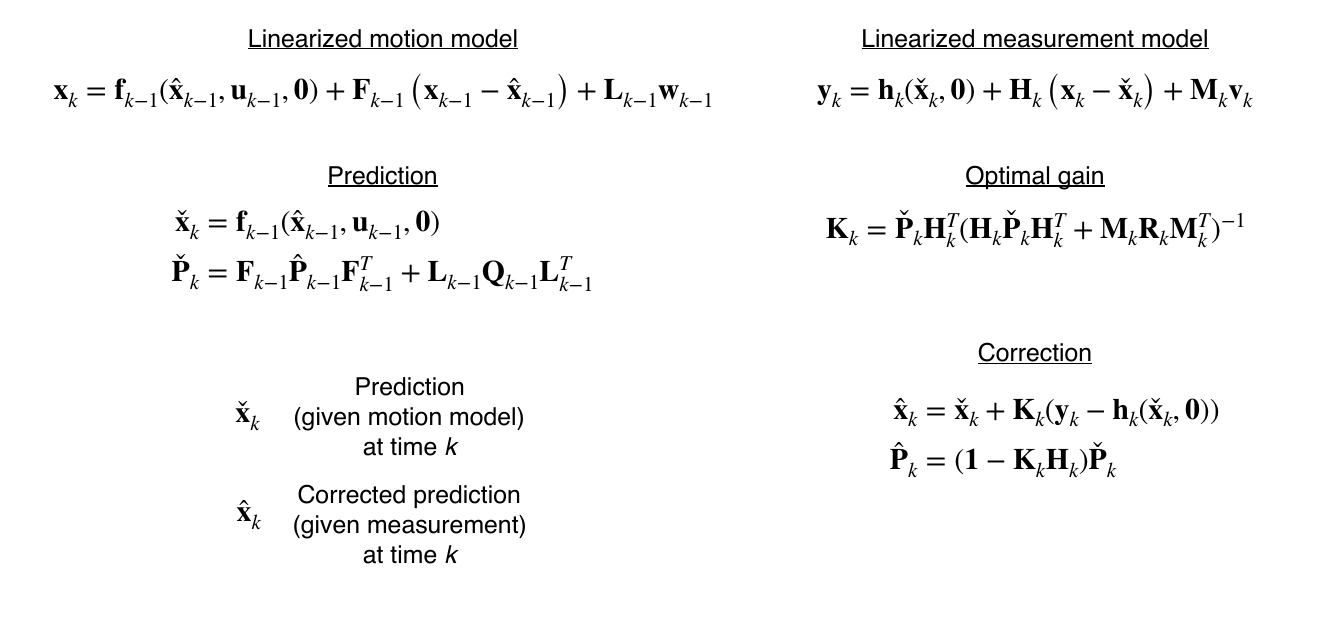
\includegraphics[scale=0.280]{img/kalman_filter/kalman_6.jpeg}
\end{center}
\caption{Summary of EKF.}
\label{kalman_6}
\end{figure}


\section{Example: EKF}
\label{example_ekf}

So, let's walk through a concrete example of actually using the EKF. We will use the same example from
module two but with a twist. We're going to track the position and velocity of a car moving along a rail. But now, instead of receiving periodic GPS measurements
that tell us our position, we're going to use an on-board sensor like a camera to measure the altitude of distant
landmarks relative to the horizon. We will keep the same linear motion model
as in the original example, and assume we know both the height of the landmark and its position
in a global reference frame. See for example Figure \ref{kalman_7}.

\begin{figure}[!htb]
\begin{center}
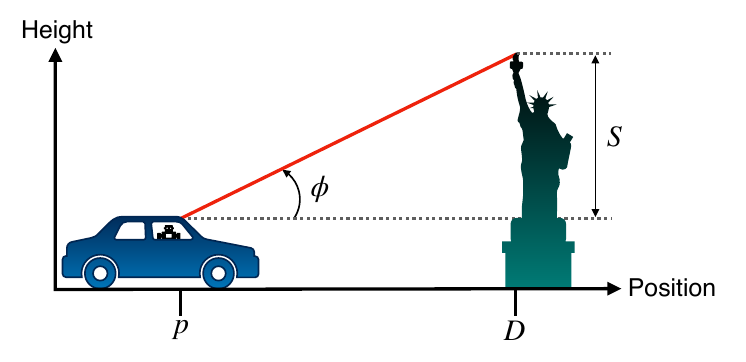
\includegraphics[scale=0.280]{img/kalman_filter/kalman_7.jpeg}
\end{center}
\caption{Summary of EKF.}
\label{kalman_7}
\end{figure}

Thus, the state vector is given by the vector

\begin{eqnarray}
\mathbf{x}_k = 
\begin{bmatrix}
p \\
\dot{p}
\end{bmatrix}
\end{eqnarray}

and it is propagated according to

\begin{eqnarray}
\mathbf{x}_k = 
\begin{bmatrix}
1 & \Delta t \\
0 & 1
\end{bmatrix}
\mathbf{x}_{k-1} + 
\begin{bmatrix}
 0 \\
 \Delta t 
\end{bmatrix}
\mathbf{u}_{k-1} + \mathbf{w}_{k-1}
\end{eqnarray}

The input signal is given by

\begin{eqnarray}
\mathbf{u} = \ddot{p} 
\end{eqnarray}

The landmark measurement model is

\begin{equation}
y_k = \arctan(\frac{S}{D - p_k}) + v_k
\end{equation}

Finally, we will use the following noise densities

\begin{equation}
v_k \sim N(0, 0.01), ~~ \mathbf{w}_k \sim N(\mathbf{0}, \begin{bmatrix} 0.1 & 0 \\ 0 & 0.1 \end{bmatrix})
\end{equation}

Because our sensor is measuring an angle, our measurement model has a nonlinear dependence on
the position of the car. We are going to need to linearize the measurement model and use it
in our Extended Kalman Filter. The Jacobians for
this problem look like this. 

\begin{equation}
\mathbf{F}_{k-1} = 
\begin{bmatrix} 
1 & \Delta t \\ 
0 & 1 
\end{bmatrix}, ~~ \mathbf{L}_{k-1} = \mathbf{I}_{2\times 2}, ~~ \mathbf{H}_k =  
\begin{bmatrix} 
\frac{S}{(D - \check{p})^2 + S^2} & 0
\end{bmatrix}, ~~ M_k = 1
\end{equation}


Notice that the $\mathbf{F}$ matrix in this problem is exactly the same as the $\mathbf{F}$ matrix
in the original problem. This is because our motion model
is already linear in the state. Also notice that
the noise Jacobians, $\mathbf{L}$ and $\mathbf{M}$, are both identity since both the emotion and the measurement
model have additive noise. 

We will be using the following data  to estimate the position of the vehicle at time one using the EKF. 

\begin{equation}
S = 20m, D= 40m, y_1 = 30 deg, u_0 = -2m/s^2, \Delta t = 0.5s
\end{equation}


\begin{equation}
\hat{\mathbf{x}}_0 \sim N(\begin{bmatrix}0 \\ 5 \end{bmatrix}, \begin{bmatrix}0.01 & 0 \\ 0 & 1 \end{bmatrix})
\end{equation}

Here is the result of the prediction step for the mean and
covariance of the state. Notice that the result is identical to the linear Kalman filter case because
the motion model actually is linear. For the correction step, this is what you should get. Keep in mind that you should use the nonlinear measurement model to
compute the measurement residual, not the linearized model. Also note that in this case, even though the corrected mean at the state estimate is different
from the predicted mean, the corrected co-variance didn't change that much from the predicted co-variance. This is because the Azimuth angle
changes slowly at this distance and doesn't provide
much information about the vehicle state compared
to a GPS measurement. 


In summary, the Extended Kalman Filter or EKF uses linearization to adopt
the Kalman filter to nonlinear systems. We will encounter several different nonlinear systems to which we can apply
the EKF or its cousin, the UKF, in the upcoming course project. Linearization works by computing
a local linear approximation to a nonlinear function using a first-order Taylor series expansion
about an operating point. This requires several Jacobian matrices which contain the set of
first-order partial derivatives. In the next section, we will discuss an
alternative formulation of the EKF called the error
state Extended Kalman Filter. This would be a useful tool later
in the course when we talk about estimating the vehicle
orientation in 3D space.

\section{Questions}


\begin{enumerate}
\item Consider the following function 
\begin{equation}
g(\mathbf{x}) = \sqrt{p_{1}^2 + p_{2}^2} 
\end{equation}
and $\mathbf{x} = (p_1, p_2, v_1, v_2)^T$ and $\hat{\mathbf{x}} = (1, 2, 3, 4)^T$. Calculate $g(\hat{\mathbf{x}})$ and $g^{'}(\hat{\mathbf{x}})$

\item Which of the following statements are true?

\begin{enumerate}
\item The ordinary Kalman filter can be used also for nonlinear models but it will be less optimal than, e.g., the extended Kalman filter. 
\item If we have a mix of linear and nonlinear models, let’s say that, e.g., the motion model is linear while the measurement model is nonlinear. 
In this case, it is appropriate to combine the Kalman filter prediction step with the EKF update step to approximate the posterior. 
\item For linear and Gaussian state space models, the EKF is equivalent to the Kalman filter. 
\item We can use the EKF for all nonlinear state space models, but it will only be accurate for “mildly” nonlinear models. 
\end{enumerate}

\end{enumerate}



\section{Assignements}
